\section{Problem III: Hydronium cation}{hydronium cation}\label{sec:problemIII}
\subsection*{Planar hydronium cation}

This exercise covers how to perform geometry optimizations.
Specifically, we will relax the H$_3$O$^+$ molecule starting from an initial planar guess for the geometry. 

\begin{enumerate}

\item Create the planar H$_3$O$^+$ geometry in geom\_planar.xyz file. Use the following coordinates:
%
\begin{table}[ht!]
\hspace*{0.5cm}
  \texttt{
    \begin{tabular}{ l S S S }
      %BL: Latest aims version has different numbers:
      %OLD
      % | Total energy uncorrected    &:    & -0.136054662652353E+02 & eV\\
      % | Total energy corrected      &:    & -0.136054662652353E+02 & eV\\
      % | Electronic free energy      &:    & -0.136054662652353E+02 & eV\\
      %NEW
      O&  0.00&  0.00&  0.00 \\
      H&  0.92& -0.53&  0.00 \\
      H& -0.92& -0.53&  0.00 \\
      H&  0.00&  1.06&  0.00 \\
    \end{tabular} 
  }
\end{table} 

\item Create a template \texttt{input.com} file, using the template provided in the first problem. Use HF and 6-31G(d,p) basis set. Moreover, we want to relax the geometry and perform the vibrational analysis of the ion. Therefore, replace the \texttt{sp} keyword ('single-point') with \texttt{opt} ('optimization') and \texttt{freq} ('frequency'). Copy the geometry of the cation at the end of the input file.  (\texttt{cat geom\_planar.xyz >> input.com} and add and empty line at the end). 


\item Run gaussian. \\ 
            \texttt{ g16 input.com \& }

\item To visualize the results, open gaussview by typing \texttt{gaussview \&} command. Select \texttt{file/open} and open the \texttt{output} file. What does the fully relaxed structure look like? Do you think that this is the structure of H$_3$O$^+$ in the gas phase? Save a picture of the ion. 

\item Select Results/Summary and note down the total energy of the ion. Next, open Results/Vibrations and you will see a list of normal modes/vibrations sorted by the wavenumber [cm$^{-1}$]. Animate some of the vibration. You should see that one of the frequencies is negative - check to what normal modes it corresponds. Write down all vibrations for the lab report and indicate to what kind of molecular motion they correspond to. 

\end{enumerate}


\subsection*{Pyramidal hydronium cation}{hydronium cation}

Next, repeat the calculations for a pyramidal hydronium cation: 

\begin{table}[ht!]
  \hspace*{0.5cm}
  \texttt{
    \begin{tabular}{ l S S S }
      %BL: Latest aims version has different numbers:
      %OLD
      % | Total energy uncorrected  &:   & -0.136054662652353E+02 & eV\\
      % | Total energy corrected    &:   & -0.136054662652353E+02 & eV\\
      % | Electronic free energy    &:   & -0.136054662652353E+02 & eV\\
      %NEW
      O&  0.00&  0.00&  0.00 \\
      H&  0.92& -0.53& -0.66 \\
      H& -0.92& -0.53& -0.66 \\
      H&  0.00&  1.06& -0.66 \\
    \end{tabular} 
  }
\end{table} 

\noindent Visualize the results with Gaussview. You should see the H$_3$O$^+$ in pyramidal conformation now.  Select Results/Summary and note down the total energy of the ion and compare it with the planar structure. Which conformation has lower energy?  Next, open Results/Vibrations to inspect normal modes/vibrations. If caclulations were done properly, all vibrations should have positive wavenumbers. Save the vibrations and descibe the motion they correspond to. 



\subsection*{Potential-Energy Surface Scan}

In the final problem, we are going to inspect the potential-energy surface of the hydronium ion along its umbrella mode. In Problem planar cation you have seen that the negative (in fact, it's imaginary, \texttt{i} is dropped by convention) frequency corresponds to such `umbrella' mode. 

\begin{itemize}
 \item Change to the \texttt{PES} directory. You will an template input file already prepared. If you open it, you should see that the xyz-cartesian coordinates has been replaced with a z-matrix. The z-matrix allows precise control of the geometry within single calculations.

\begin{table}[ht!]
  \hspace*{0.5cm}
  \ttfamily{
    \begin{tabular}{ l l  l l }
      
      O&  	  & 	     &       \\
      X&  1 a	& 	     &       \\
      H&  1 a &  2 HOX &       \\
      H&  1 a &  2 HOX & 3  120.0 \\
      H&  1 a &  2 HOX & 3 -120.0 \\

      a=OH \\
      HOX= 135. -1. 45 \\
      $[$ empty line $]$
    \end{tabular}
  }
\end{table}  

\begin{figure}
\begin{center}
 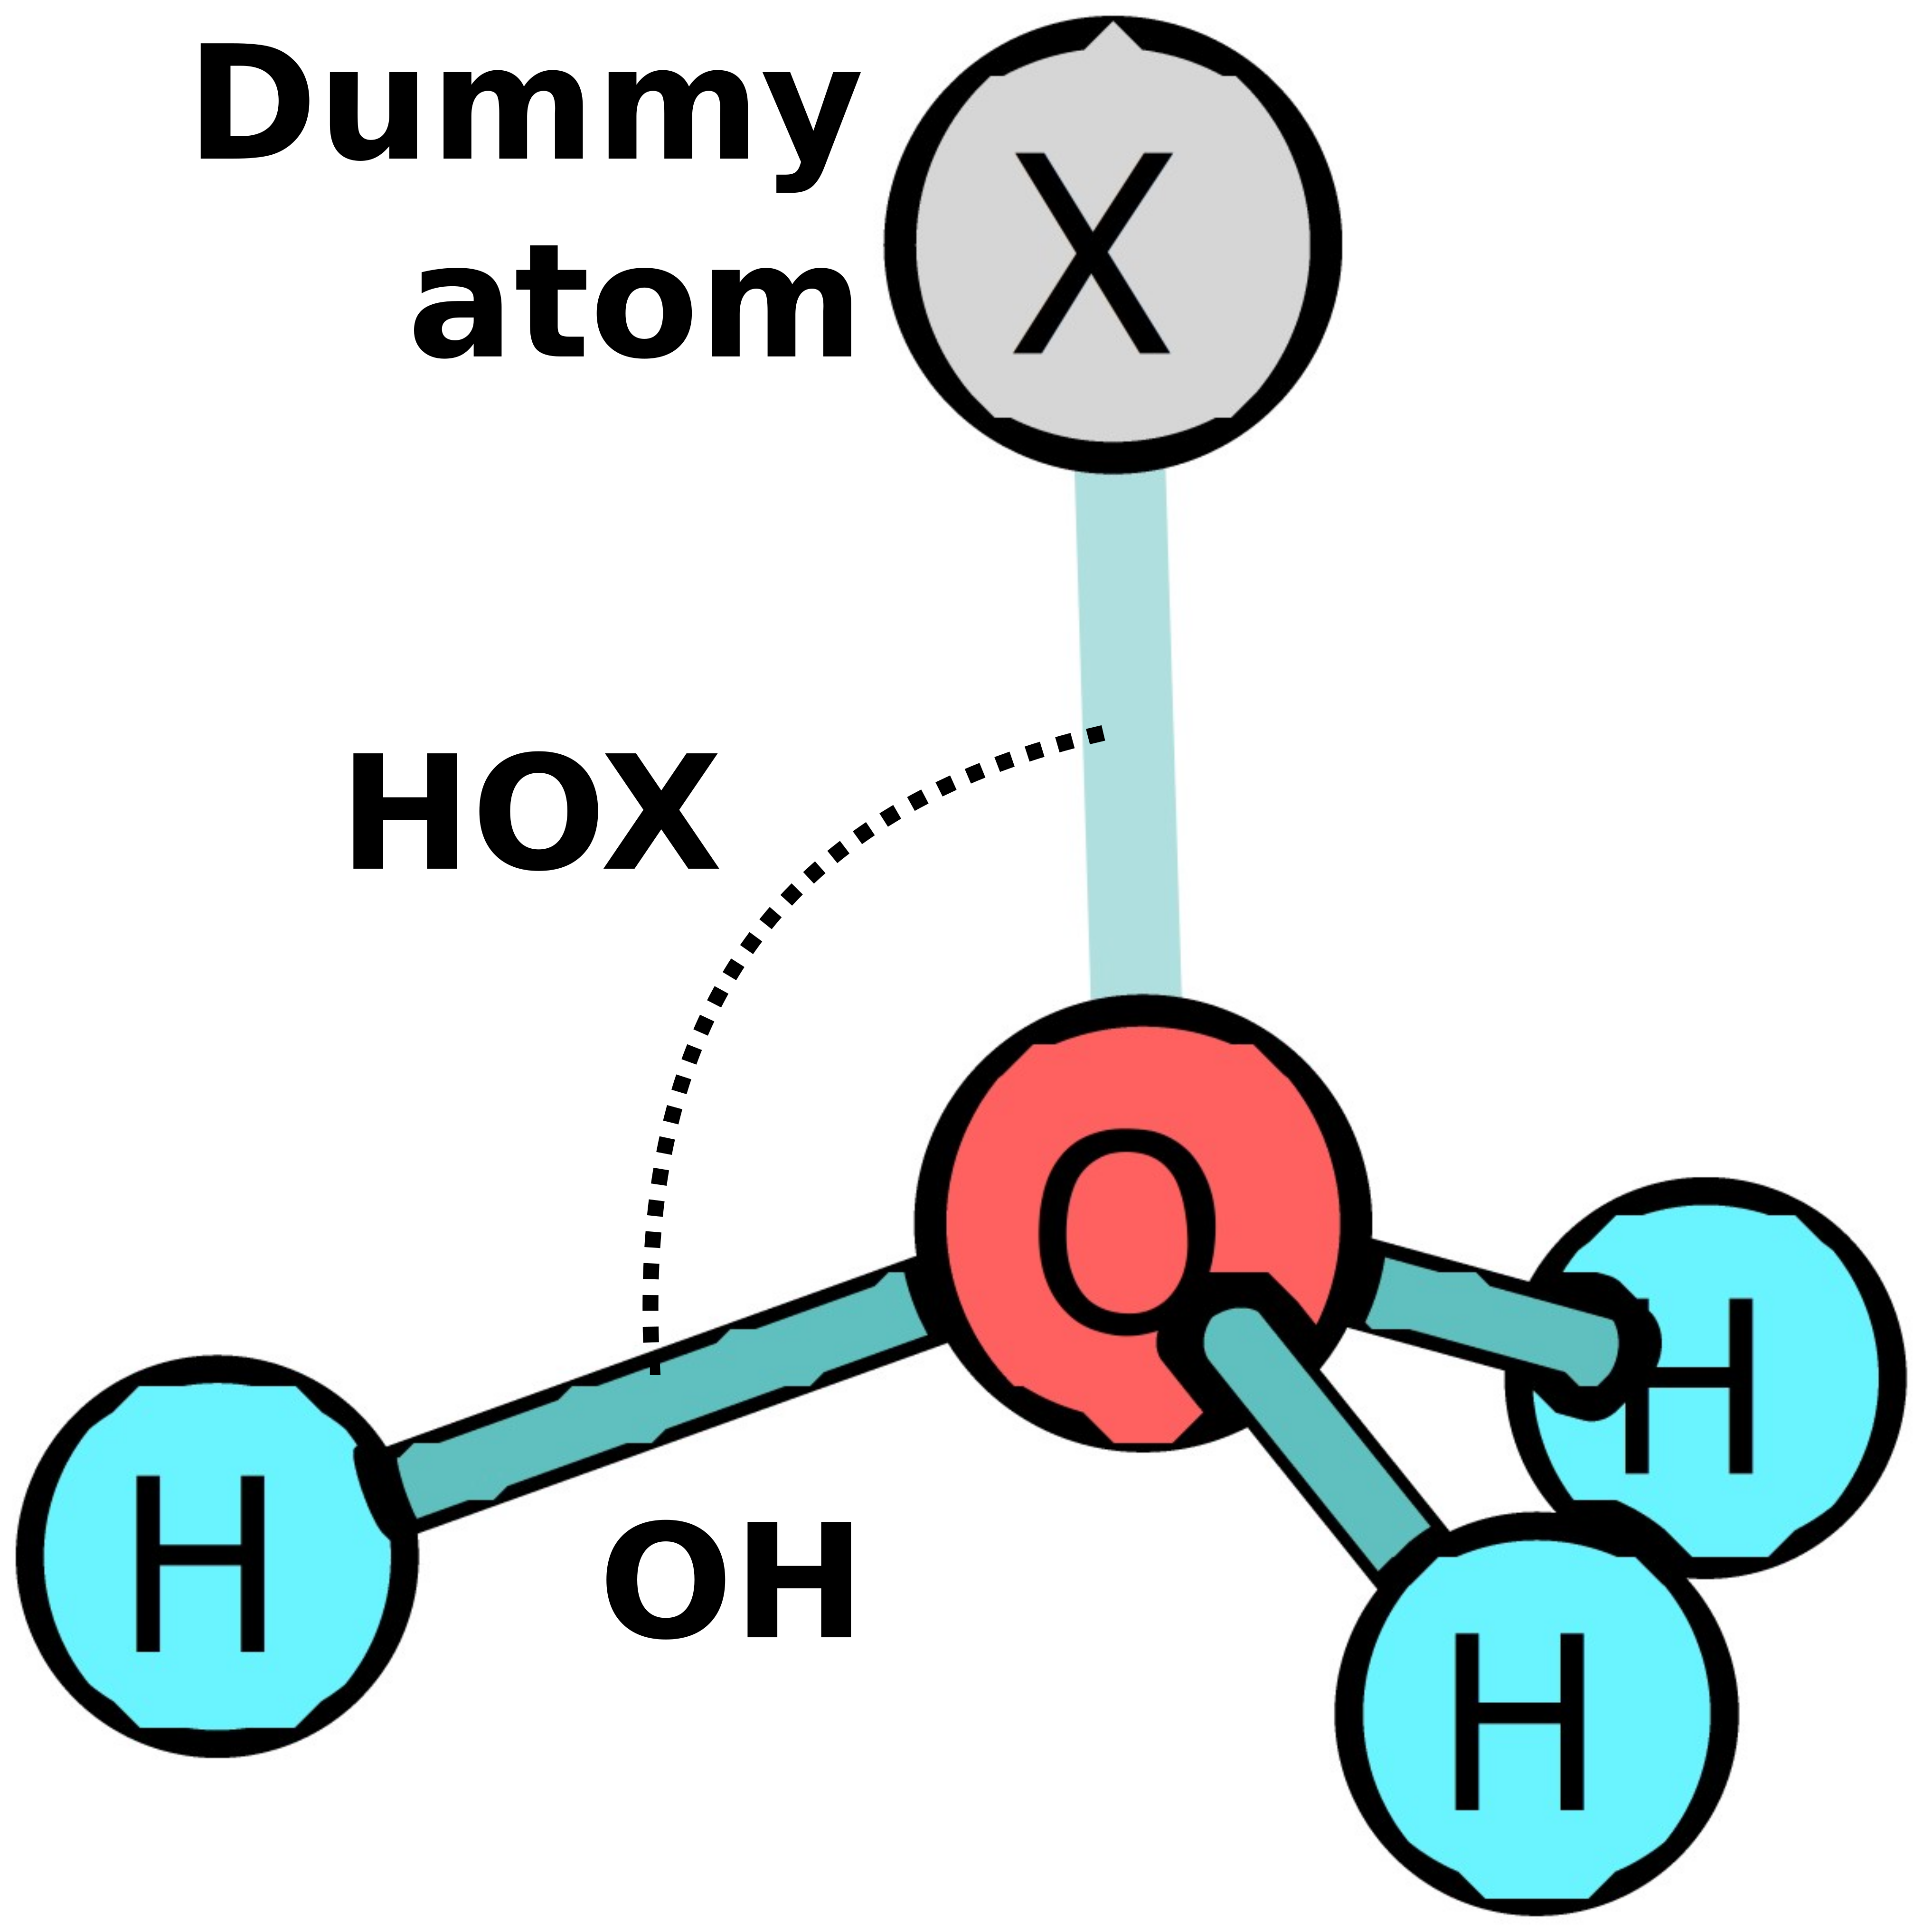
\includegraphics[width=0.3\textwidth]{pics/zmat.png}
 \end{center}
 \caption{ Definition of hydronium ion internal coordinates. The calculations perform a scan along HOX coordinates for all 3 hydrogens between 135 and 90 degrees. 120 degrees dihedral angle indicates the relative position of hydrogen atoms. }
\end{figure}


\item The first column shows the bonding, second shows the angles between atoms and the third column specifies the dihedral angle. X is a dummy (non-existent) atom that enables to control the umbrella motion. Figure below explains the z-matrix graphically. First, open the optimized pyramidal ion and measure the O-H distance and replace \texttt{OH} in the input file. Next, run the calculations. The calculations will perform a scan along the X-O-H angle, performing a single point calculations every 1 degree from 135 to 90 degrees. When the calcualtions are finished, visualize the results with gaussview (results/scan). Save the results, the Potenstial-Energy Surface (PES) along the specified coordinate (X-O-H angle). The PES for angles below 90 degrees is the mirror image. Use kcal/mol instead of Ha in the report. 

\item Localize the lowest-energy and transition structure along the PES and calculate the reaction barrier of the internal flip of the hydronium ion. Whereas the energy of the pyramidal ion is comparable with the minimum on the PES, the energy of the optimized planar cation and the maximum on PES is different. Why? Compare the geometries. 

\item In the final step, rerun the calculations using \texttt{MP2} method. 


\end{itemize}

\section*{Lab report}

For the lab report, please prepare following data. This is bare minimum, there are couple of open questions in the text that you should try to asses. 

\begin{enumerate}
 \item Plot the Energy vs number of basis function for a hydrogen atom for all methods used in problem 1. 
 
 \item Plot the binding curves for HF using Hartree-Fock and PBE1PBE methods. Find the minimum distance and compute the atomization energy. Plot the dipole moment as a function of the bond distance. 
 
 \item Prepare tables listing molecular vibrations in hydronium ion in planar and pyramidal geometries. Assign the wavenumbers to molecular vibrations. 
 
 \item Plot the PES along the HOX coordinate using HF and MP2 methods. Use kcal/mol for the y-axis. Compute the heigh of the barrier separating two pyramidal structures. 
  
\end{enumerate}


